\section{Data Analysis}
\label{sec:Analysis}
%In this work we analyse the data from \Xehund's scientfic run II~\cite{xe100_run10_si,xe100_run10_sd} recorded between February 2011 and March 2012, 
In this work we perform a re-analyse of the scientfic run~II data recorded between February 2011 and March 2012, 
corresponding to 224.6~live~days.\RanComment{ A calibration sample is obtained to characterize the detector response to NR and ER interactions, as well as for estimating the background from $\beta$ and $\gamma$-particles. For the ER sample we expose the detector to $^{60}$Co and $^{232}$Th sources, while for the NR sample we use $^{241}$AmBe.} \textcolor{red}{Some words about calibration data used}.

This analysis extends the previous results~\cite{xe100_run10_si,xe100_run_combination}, addressed in the following as the low energy channel , with a new study exploring the energy range between 30-180\,PE (43-240\,keV \RanComment{Make sure this value is correct!!!}) in $S1$  \textcolor{red}{maybe better to say in KeV??}. 
%However we enlarge the energy range to be 3PE-180PE. In order to preform a blind analysis we divide our work into two energy ranges. Low energy , 3PE-30PE which is identical to the range in the works mentioned above, and a high energy range, 30PE-180PE. The main emphasis of this paper is the second region, on which no work has been done yet. 
\RanComment{There is a bit of repetition in these two paragraphs consider revising }The data analysis is divided into two mutually exclusive channels, one optimized for low energies and ranging from 3-30\,PE in $cS1$ \RanComment{(LowE)}, the other optimized for high energies recoils
ranging from 30-180\,PE in $cS1$ \RanComment{(highE)}, which are finally statistically combined. 
The relative region of interests (ROI) of these two channels are shown in Figure~\ref{fig:phasespace} and further described in the following sections. 

\RanComment{Not sure this paper is so long we actually needs this full description, In any case I believe it is important to state the main new thing of this analysis which is the high energy part}
This section describes the analysis procedures such as selection criterion, background expectation models and signal acceptance estimation  employed
for the low and high energy channels, reported in Section~\ref{subsec:LowE} and~\ref{subsubsec:HighE} respectively. 
%This work focuses on the high energy channel, a brief description of the low evenrgy channel is reported in Section~\ref{subsec:LowE}.
\RanComment{I think maybe we should explain the S2 bottom used (might go in signal model or here)}

\subsection{Low Energy Channel}
\label{subsec:LowE}
This analysis channel relies on the re-analysis of run~II data described in~\cite{xe100_run_combination}. The region of interest (ROI), the background 
expectation models, data selections and their acceptances are mostly unchanged and so are only briefly summarized here. Differences with respect to said results are highlighted when present.

The ROI for this channel is defined in the ($y,cS1$)-plane and is shown in Figure~\ref{fig:phasespace}.  The lower 
bound on $y$ corresponds to a 3\,$\sigma$ acceptance quantile (as a function of cS1) of a 20~GeV WIMP mass signal model assuming an $\mathcal{O}_1$ (SI) interaction, while the upper bound is fixed at y\,=\,2.7.
The range in cS1 is selected as 3 to 30\,PE. 
The ROI is further divided into eight sub-regions (also called bands) depending on the operator $\mathcal{O}_i$ and on the WIMP mass hypothesis. 
These bands are arranged to achieve constant expected signal density in each region, as described in~\cite{xe100_run_combination}.

\begin{figure}[]
\begin{minipage}{1\linewidth}
\centerline{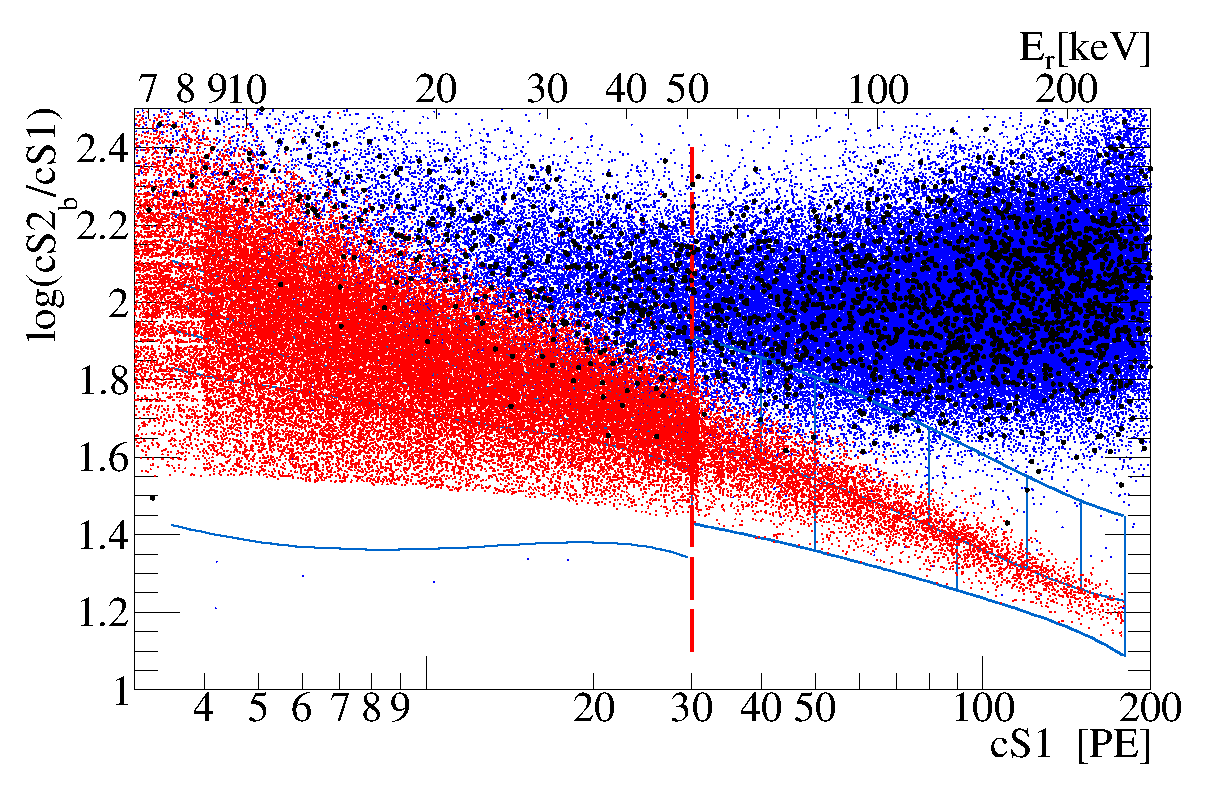
\includegraphics[width=1\linewidth]{Figures/eft_sr.eps}}
\end{minipage}
\caption{Summary of regions of interest, backgrounds, and observed data. ER calibration data, namely $^{60}\mathrm{Co}$ and $^{232}\mathrm{Th}$ data is shown as blue dots. NR calibration data ($^{241}$AmBe) is shown as red dots. Dark matter search data is shown as black dots. The red dashed line is the threshold between the low and high energy channels. The lines in blue are the bands. For the low-energy channel these are operator and mass dependent, but are shown here for a 50~GeV/$c^2$ WIMP using the $\mathcal{O}_1$ operator. For the high-energy region, the nine analysis bins are presented also in blue lines.
%\sout{the top left bin in this region is bin 1, the top right is bin 6, the bottom left is bin 7 and bottom right is bin 9. 
%In Sec.~\ref{sec:Results} we show similar data but for regions above the upper range of this analysis, going up to 1000\,PE in cS1, for completeness as part of final unblinding of XENON100 data.} 
}
\label{fig:phasespace}
\end{figure}  


Other than falling into the ROI, an event should fulfill several additional selection criteria (cuts). Data quality and selection cuts are defined to remove events with poor data quality or noisy signals. \ale{Events are discarded if they present} a time-coincident signal in the outer LXe veto, S2 signals below threshold, multiple-scatters, or are localized outside a predefined fiducial volume of 34 kg. In addition, this analysis channel uses the post-unblinding cuts and data reprocessing described in~\cite{xe100_run_combination}. More details on these selection criteria and their relative WIMP signals acceptances can be found in~\cite{Aprile:2012vw,xe100_run_combination}. 
%%%%% MAYBE THIS CAN BE COMMENTED OUT %%%%%%
%%% Ale : already sayd above, and is not "new features" of this analysis.
%\sout{To summarize the main new features in this analysis, data is reprocessed with an improved (S1,S2) classification algorithm, and a new cut targeted to suppress data periods with non-random occurrence of lone-S1 (an S1 without 
%any correlated S2) events is applied.} 
%%%%%%%%%%%%%%%%%%%%%%%%%%%%%%%%%%%%%%%%%%%%%
\ale{Note that}
%Finally, 
this analysis channel does not employ a variable lower S1 threshold as a function of the event position in the TPC, but instead applies a fixed lower threshold cut on cS1 at 3\,PE, \ale{conversely} to the choice made in~\cite{xe100_run_combination}.

The expected background is modeled separately for ER and NR contributions which are then scaled to exposure and added together.
The NR background is estimated by Monte Carlo simulation and accounts for the radiogenic and cosmogenic neutron
contributions~\cite{Aprile:2013tov}. The ER background is parametrized as the linear combination of Gaussian-shaped and non-Gaussian components.
The first is obtained via a parametric fit of the $^{60}$Co and $^{232}$Th calibration data, as discussed in~\cite{xe100_run10_si}.
%In contrast, the expected distribution and yields for the non-Gaussian population, 
\ale{The second, } consisting of anomalous events such as those 
presenting incomplete charge collection or accidental coincidence of uncorrelated S1s and S2s,  
is evaluated via dedicated techniques described in~\cite{xe100_run_combination}.

\ale{Systematic uncertainties on the background model arising from the Gaussian parametrized fit, from the normalizations of the NR and from the non-Gaussian components, have been evaluated and propagated to each band}. \BenComment{*This sentence doesn't make sense; missing an "and" or something? I can't quite guess what it is supposed to mean*} These errors are small with respect to the statistical uncertainties of each band, which are conservatively taken as the overall uncertainty~\cite{xe100_run_combination}, as discussed in Sec.~\ref{sec:LikelihoodFunction}.



\subsection{High Energy}
\label{subsubsec:HighE}

%\subsection{Analysis and Data Selection}
%\subsection{Data Selections}
%\label{subsec:AnalysisAndDataSelection}

The data selection cuts which are defined to low energy recoil only, are extended, modified or removed to be compatible with high energy recoils. Most of the cuts were fully compatible or simply extended to high energy depositions, however \sout{one cut is dropped and two are modified} \RanComment{some required a more comprehensive study}. In order to throw away peculiar events we compare the width of the S2 to its z-position. In this analysis we adopt a newer version of this cut, developed for scientific run III see ~\cite{xe100_run_combination}. As a WIMP will interact only once in the detector we remove events whcih have more then one S2. we adopt here a cut that is more suitable to higher energies and demands a single S2 in a 160 $\mu$S window. In order to define the interaction exact location, we use several algorithms, one of the is the Neural Network (NN), as we do not train the detector using high ER events, the NN gives a large $\chi^2$ for these events. In order to not under estimate the background we drop this cut. We do keep other cuts on position reconstruction to make sure we can fiducialize correctly for more details on all cuts see ~\cite{xe100_ana2012}. Finally the total acceptance is fitted using a 3rd order polynomial presented in Figure~\ref{fig:Acc}

\begin{figure}[h!]
\begin{minipage}{1.\linewidth}
\centerline{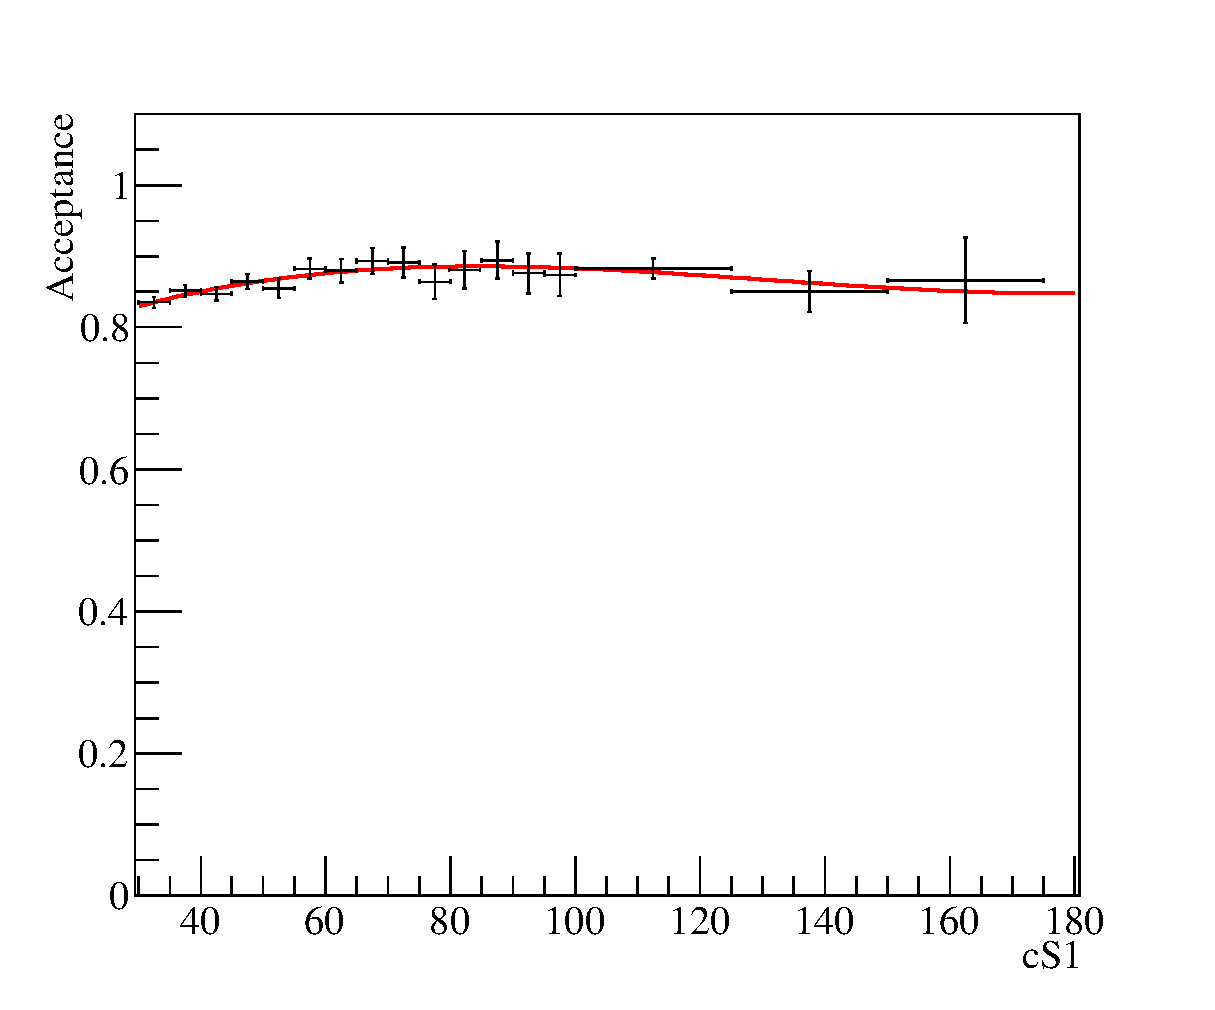
\includegraphics[width=1.\linewidth]{Figures/Acceptance.eps}}
\end{minipage}
\caption{The total acceptance of all cuts used, data from calibration in black and the fit in red.}
\label{fig:Acc}
\end{figure}

We define our signal region in the discrimination (y,S1)-plane using $^{241}$AmBe calibration data. The upper bound is defined such that the ROI is not contaminated from contribution due to xenon exitation lines.
The lower is defined as the 3\,$\sigma$ acceptance quantile of the NR distribution, this is done for preventing gamma-X events to penetrate the sample.

We divide our signal region into two bands in log(S2/S1). The bands are constructed such that the NR data sample is equally distributed between them, in each band there are $\sim3000$. Each band is divided into several bins. The definition and content of each bin is presented in table~\ref{table:BinDef} and in Figure~\ref{fig:phasespace}. 


%%%%%%%%%%%%%%%%%%%%%%%%%%%%%%%%%%%%%%%%%%%%%%%%%%%%%%%%%%%%%%%%%%%%%%%%%%%%%%%%%%%%%%%%%%%%%%%%%%%%%%%

%%%%%%%% THIS PROBABLY NEEDS A SECTION, explaining well the uncertainty determination %%%%%%%%%%%%%%%%%
The main source of background is coming from ER leakage and hence, we estimate our background using calibration sample defining the distribution between the bins. 
\RanComment{Contribution from radiogenic(what's the correct spelling???) neutrons and accidental coincidence are negligible for such a high energy recoil .}
For sensitivity estimation we calculate a normalization factor in a sideband. For the final overall normalization we let the scaling factor be a free parameter to best fit the data.
%%%%%%%%%%%%%%%%%%%%%%%%%%%%%%%%%%%%%%%%%%%%%%%%%%%%%%%%%%%%%%%%%%%%%%%%%%%%%%%%%%%%%%%%%%%%%%%%%%%%%%%


\begin{table}
\resizebox{\columnwidth}{!}{

	 \begin{tabular}{|c| c| c| c| c| c |} 
 \hline
 Bin Number & Band  & Energy Range (cS1)  & \# Background Events & \# Data Events \\  
 \hline\hline
 1 & upper & 30  - 40  & 23.5 & 20 \\ 
 \hline
 2 & upper & 40  - 50  & 15.7 & 17 \\
 \hline
 3 & upper & 50  - 80  & 12.4 & 11 \\
 \hline
 4 & upper & 80  - 120 & 1.1  & 1  \\
 \hline
 5 & upper & 120 - 150 & 0.1  & 1  \\  
 \hline
 6 & upper & 150 - 180 & 0.08 & 0  \\  
 \hline
 7 & lower & 30  - 50  & 0.9  & 0  \\  
 \hline
 8 & lower & 50  - 120 & 0.35 & 0  \\  
 \hline
 9 & lower & 120 - 180 & 0.18 & 0  \\  
 \hline
\end{tabular}
}

\caption{Bins definition. The estimated background event is calculated by taking the calibration sample and scaling it by $6.54\times10^{-3}$, which is a the ration between data and calibration in a sideband. The number of data events is the number of events from the DM data set in each bin.\textcolor{blue}{I changed this table as well a bit}} \label{table:BinDef}

\end{table}


\begin{figure}[h!]
\begin{minipage}{1.\linewidth}
\centerline{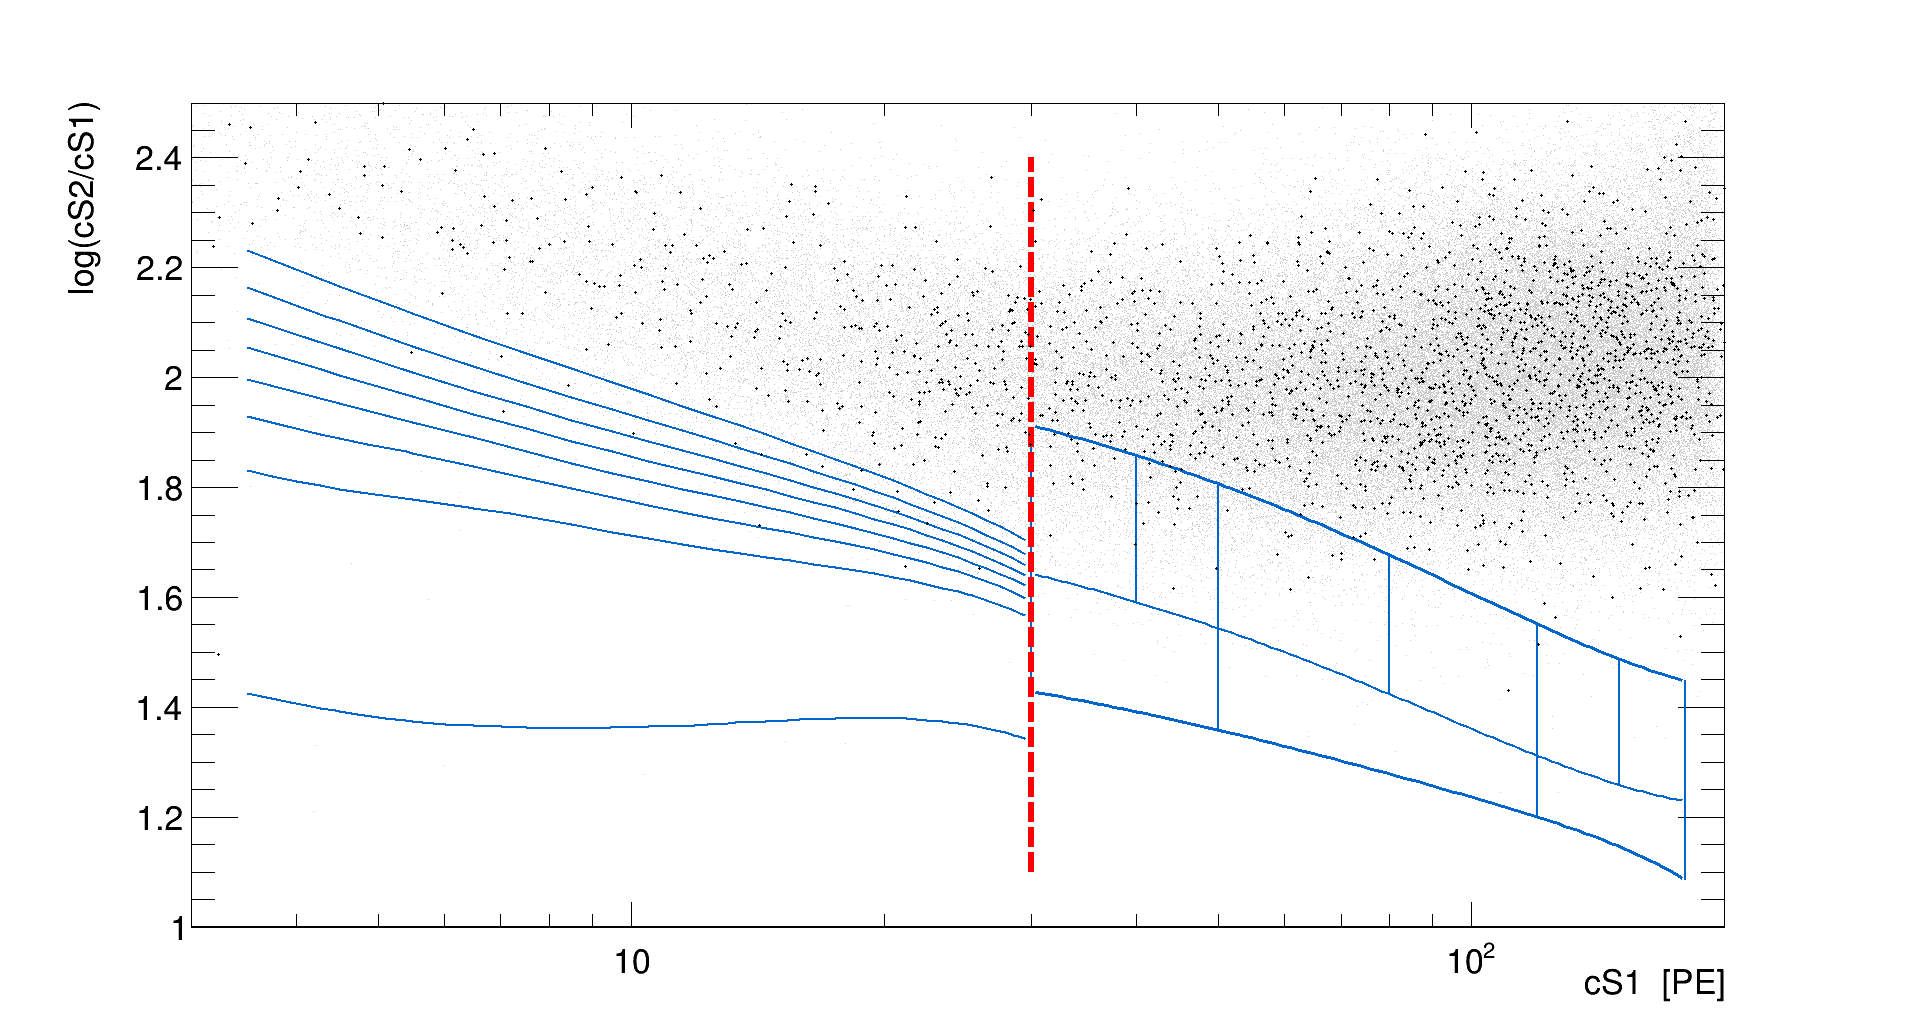
\includegraphics[width=1.\linewidth]{Figures/eft_sr.png}}
\end{minipage}
\caption{$^{60}\mathrm{Co}$ and $^{232}\mathrm{Th}$ data in light gray and DM data in black dots. The red line is the threshold between the lowE part and the highE one. In blue are the bands. For lowE constructed using data from a 50 GeV/$c^2$ WIMP. For the highE region the 9 bins are presented. top left is bin number 1,  top right is bin number 6, bottom left is bin number 7 and bottom right is bin number 9.}
\label{fig:phasespace}
\end{figure}  




\subsection{Signal Model}
\label{subsec:SignalModel}
In order to estimate the energy deposition in the high E region we use the \Leff\ based method which is given in Eq.~\ref{eq:LeffEnergyScale}
\begin{equation}
\label{eq:LeffEnergyScale}
	E_{nr} = \frac{cS1}{L_y} \frac{1}{L_{eff}(E_{nr})} \frac{S_{ee}}{S_{nr}}
\end{equation}
The energy range in this region is bounded by the statistics of NR calibration data, namely $^{241}$AmBe.

The signal model is then produced by taking the event rate spectra converting it to S1, applying the acceptance and the detector response (explained in ~\cite{xe100_ana2012}) to give the expected event rate in the detector for each operator see Figure~\ref{fig:HighE}.
\begin{figure}[h!]
\begin{minipage}{1.\linewidth}
\centerline{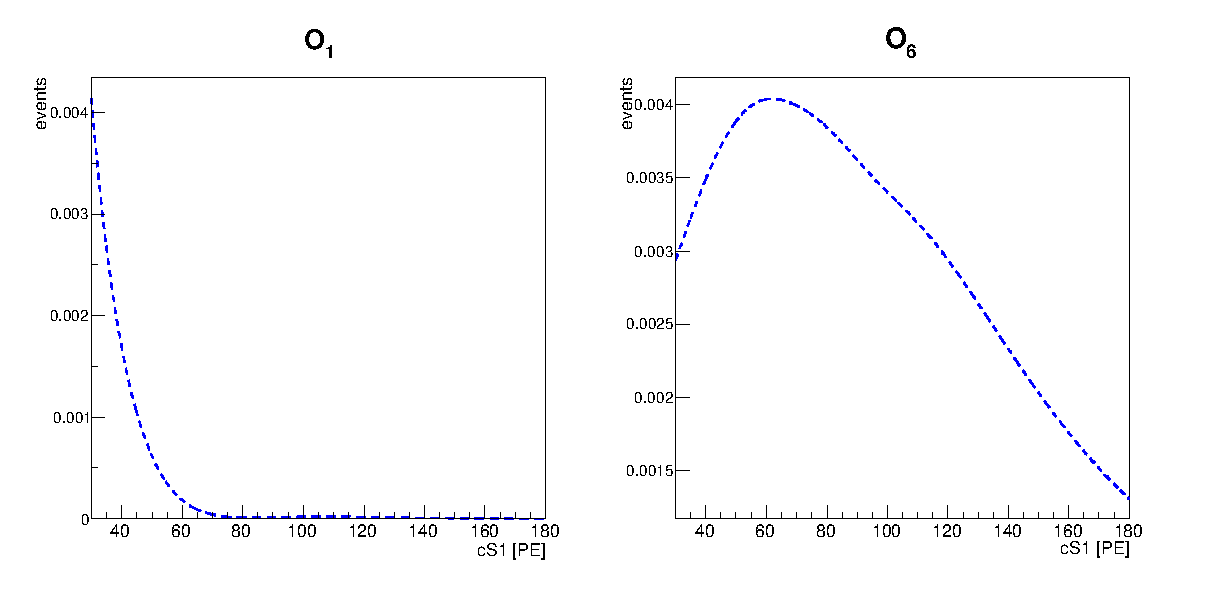
\includegraphics[width=1.\linewidth]{Figures/SigHighO1O6.eps}}
\end{minipage}
\caption{The expected signal in the high energy region for a 300 GeV/$c^2$ WIMP mass, Normalized to 5 events. Left(right) is the spectra for $O_1$($O_6$). Notice that for $O_1$ most of the events are not expected to deposit energy higher then 30 PE whereas for $O_6$ a large fraction of the events appear in this region.}
\label{fig:HighE}
\end{figure} 




\textbf{Ben add here} For the low energy region ...explain shortly the 2D signal model, and give ref to run combination paper. In fig~\ref{fig:LowE} is an example of the expected signal for $O_1$ and $O_6$ normalized to give 5 events in the total energy range (low E and high E)
\begin{figure}[h!]
\begin{minipage}{1.\linewidth}
\centerline{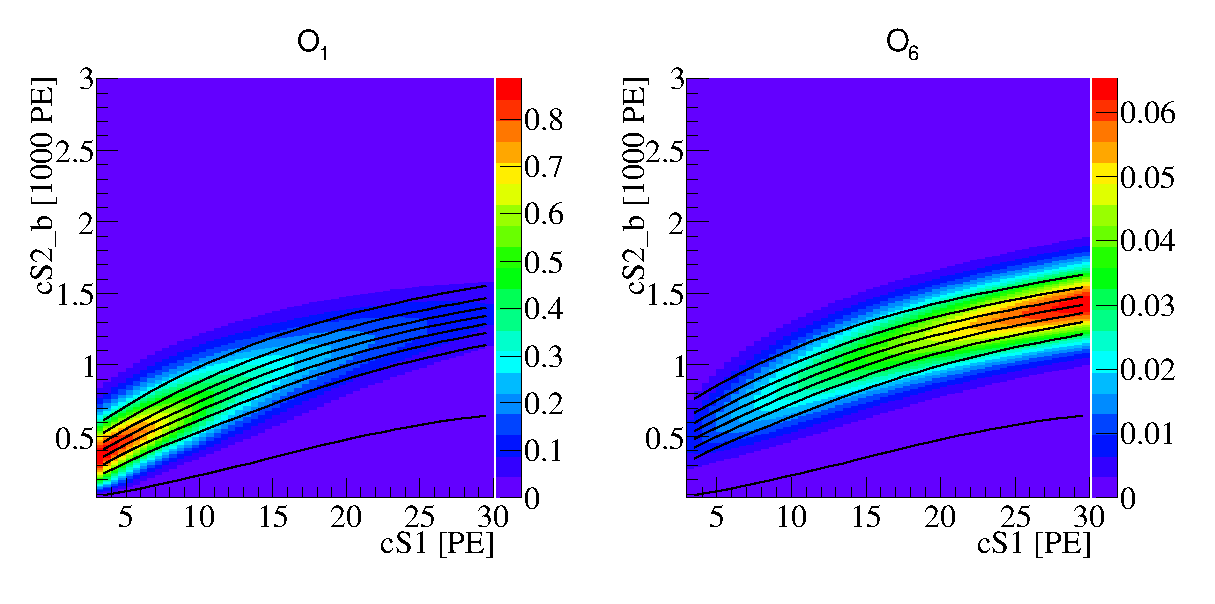
\includegraphics[width=1.\linewidth]{Figures/SigLowO1O6.eps}}
\end{minipage}
\caption{The expected signal in the low energy region for a 300 GeV/$c^2$ WIMP mass, Normalized to 5 events. Left(right) is the spectra for $\mathcal{O}_1$($\mathcal{O}_6$). Notice that for $\mathcal{O}_1$ most of the events are expected to deposit energy lower then 30 PE whereas for $\mathcal{O}_6$ a large fraction of the events do not appear in this region at all.}
\label{fig:LowE}
\end{figure}





\subsubsection{Elastic Scattering}
\label{subsubsec:Elastic}
Explain here how to get drde etc. give ref to fitzpatrick
\subsubsection{Inelastic WIMP Scattering}
\label{subsubsec:Inelastic}
explain the obtaining of inelastic and give ref to chang
